\Section{2 DoF model}

\Subsection{Non-dimensional equations of motion}

\par The model chosen for this simulation is a simple two degree of freedom, two dimension, point mass model. 
The aircraft is assumed to be a glider to simplify the optimization routine. 
With such assumption the equations of motion in the ground reference frame is :

\begin{equation}
	\begin{array}[c]{c}
		\ddot{x}= -L' \cdot sin(\gamma) + D' \cdot cos(\gamma) \\ 
		\ddot{z}= L' \cdot cos(\gamma) - D' \cdot sin(\gamma) - m \cdot g
	\end{array}
	\label{eqn:eqm}
\end{equation}

% should I include a figure with the reference frame, and angle definition?

\par The lift and drag are defined are: 

\begin{equation}
	\begin{array}[c]{c}
		L'= \frac{1}{2} \rho V^2 C_l \\ 
		D'= \frac{1}{2} \rho V^2 C_d 
	\end{array}
	\label{eqn:Cl_def}
\end{equation}

\par With $V$ being the relative wind for the vehicle.
% do I need to include this kind basic stuff?

\par Since this simulation is mainly concerned with Newtonian physics (rather than fluid phenomenons) the usual fluid dynamics non-dimensional variables make little sens.
Here the equations are normalized by the optimal glide speed and $g$, the gravitational acceleration.
This is more representative of the performances of the aircraft.

\par Following Lissaman's \cite{lissaman2005wind} implementation of the equation of motion we define $V^*$ the optimal glide speed for the aircraft. This speed is achieved at the optimal lift to drag ratio of the aircraft.
With $C_l^*$ and $C_d^*$ the angle of attack for the maximum lift to drag ratio and $\gamma$ the pitch angle with respect to the horizon the optimal glide speed is:

\begin{equation}
	\begin{array}[c]{c}
		\gamma^*= - atan(\frac{C_l^*}{C_d^*}) \\
		V^* = \sqrt{\frac{2mg}{\rho S (C_l^* cos(\gamma^*) - C_d^* sin(\gamma^*)}}
	\end{array}
	\label{eqn:glide_speed}
\end{equation}

\par From this we define $U$ and $W$ the non dimensional horizontal and vertical speed in the inertial reference frame.

\begin{equation}
	\begin{array}[c]{c}
		U = \frac{\dot{x}}{V^*} \\
		V= \frac{\dot{z}}{V^*}
	\end{array}
	\label{eqn:non_dim_speed}
\end{equation}
The time is normalized by $g / V^*$.

\par Since the speed is seen as a fraction of the optimal glide speed it makes sens to also normalize the lift and drag coefficients by their corresponding values at the optimal lift to drag ratio.

\begin{equation}
	\begin{array}[c]{c}
		L= \frac{C_l}{C_l^*} \\
		D= \frac{C_d}{C_d^*} 
	\end{array}
	\label{eqn:non_dim_coef}
\end{equation}

\par Finally we introduce Q the dynamic pressure as:

\begin{equation}
	Q = \frac{L'}{MgL} = \frac{\frac{1}{2} \rho V^2 C_l C_l^* }{Mg}
	\label{eqn:dynamic_pressure}
\end{equation}

\par From there the equation of motion \ref{eqn:eqm} can be expressed as:

\begin{equation}
\begin{array}[c]{c}
	\frac{dU}{dT}= -LQ \cdot sin(\gamma) + DQ \cdot cos(\gamma) \\ 
	\frac{dW}{dT}= LQ \cdot cos(\gamma) - DQ \cdot sin(\gamma) - 1
	\end{array}
	\label{eqn:non_dim_eqm}
\end{equation}

With 

\begin{equation}
	\gamma = -atan(\frac{W}{U})
	\label{eqn:gamma_def}
\end{equation}

\par Finally the remaining thing to consider is $Q$ the dynamic pressure. If we define the speed of the wind gust as $W_g$ and $U_g$ we can express:

\begin{equation}
	Q = V^2 = (W-W_g)^2 + (U-U_g)^2
	\label{eqn:q_def}
\end{equation}

\par With these definitions we have the basic formulation of our non-dimensional equation of motions, normalized by the performances at the optimal glide trajectory in a calm environment.

\Subsection{Lift and drag models}

\par The normalized equation of motion \ref{eqn:non_dim_eqm} are not accounting for the fluid dynamic part of the flight.
The most important factor for glide performance is the lift to drag ratio. 
In his paper, Lissaman \cite{Lissaman2007neutral} is using a relatively simple quadratic model for the relationship between lift and drag:

\begin{equation}
	D=\frac{Q}{2G}(1+L^2)
	\label{eqn:Lissaman_G}
\end{equation}

[CHECK THIS EQUATION !!!!!]

\par This simple model work relatively well for simple airfoil but is inadequate for more complex shapes.
For various reasons, small UAVs tend to have non classical designs such as blended wing body or flying wing shapes.
The advantages of these designs reside in bigger space available for the payload while keeping the drag low.
However the flying wing airfoil profiles have very different lift to drag characteristics compared to more classical airfoils.

\par To get the lift to drag curve of a typical flying wing a typical flying wing shape is tested in the XFLR5 software.

%\par [FIGURE OF THE UAV !!!]
\begin{figure}[ht]
	\begin{center}
  \scalebox{0.5}            % rescale the figure by a factor of 0.8
  {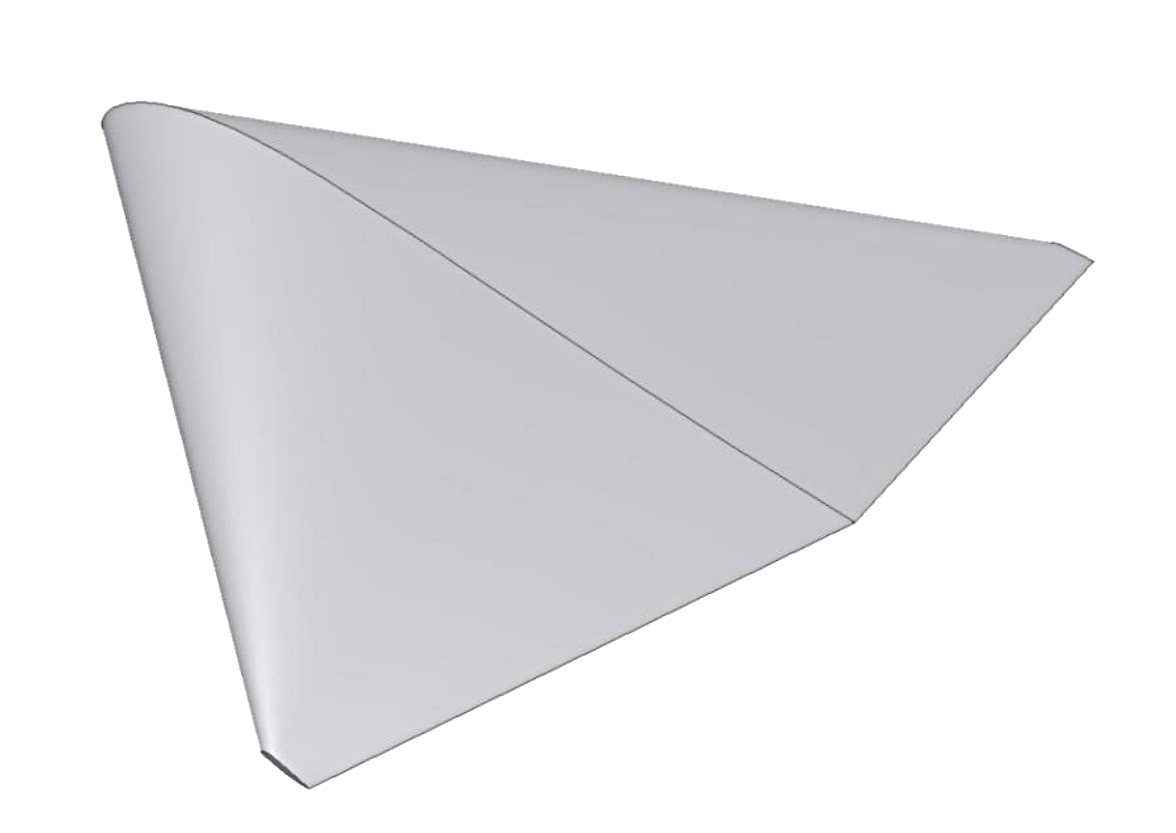
\includegraphics{./Figures/UAV.png}}
	\end{center}
	\caption{Flying wing UAV shape used in XLFR5}
	\label{fig:UAV}
\end{figure}


\par This software perform flow simulation over the aircraft with a panel based method. 
The simulation is performed on a range of angle of attack from negative XXXX degrees to to separation at XXXX degree.
Due to the presence of sharp edges at the tip of the wings the Reynolds number had to be limited to XXXX.
At each angle of attack the software automatically computed the steady lift and drag coefficients.

\par [GRAPH OF CL AND CD VS ALPHA !!!]

\par This results, while being arguably more realistic than a simple quadratic approach, are still only considering quasi-steady change in the angle of attack.
This limitation will be discussed more in depth in the result discussion section \ref{sec:results}.


\Section{Optimization process, cost function and constraints}

\Subsection{General consideration on optimization}
% Get some stuff from the MM544 class

\par The general principle for the optimization routines resides in defining a so called ``cost function'' that will represent a quantity we want to minimize.
While the algorithm tries to minimize this scalar, a series of constraints have to be respected. 
These constraints can represent physical limitations or system requirements.
The cost and constraints are expressed as functions of a set of system state variables.
The state variables can represent temporal or spatial values.
The optimization is performed in a sequential fashion where different algorithm are used to step from a set of values for the state variables to another. 

\par Optimization routines are divided into two families. 

\par The first method is the gradient method, it requires a good knowledge of the physics behind the problem.
The cost function as well as the constraints have to be explicitly defined.
In this method the gradient of the cost function and the constraints is used to determine the direction of the next step in the optimization.
Different algorithm are used to chose the step size, and sometime the direction of the previous step can influence the current step.
The gradients for either the cost function or the constraints do not have to be explicitly defined as modern optimization routines, such as the one included in Matlab, can perform numerical gradient estimation.
However putting user calculated gradient into the routine will significantly speed up the overall calculation.

\par The second method is using the so called ``evolutionary algorithms''. 
This method relies a lot less on knowing the underlying physical phenomenon.
Its basic principle is a ``try and see'' process.
Random changes are performed on the state variables and their effects on the cost function are assessed.
The best steps are selected as a starting point for the next generation.
While with this method each step is a lot less computation intensive than with the previous method, the number of steps is a lot higher.

\par The first method has been used in this optimization as it provides more insight on the physics behind the problem.
However it should be noted that the resulting ``optimal'' point is usually only assured to be \emph{a local} minimum of the cost function.
Several different starting states should be tested to ensure that the optimization converges toward a reasonable minimum.



\Subsection{Cost function}
\par Our problem here consists in optimizing the trajectory in a gusting environment to minimize energy lose.
The most obvious cost function would be something like

\begin{equation}
	- \frac{1}{2}m{V(T_f)}^2 - gX(T_f)
	\label{eqn:eni_cost_fun}
\end{equation}

Which would be equivalent to maximizing the total energy at the end of the gust.
However after testing this has shown to leave to much freedom to the algorithm. 
As a result the local minimum found are the result of trajectories such as very steep dives, clearly far from the optimum.

\par Once again we refer to the Lissaman paper \cite{Lissaman2007neutral} and chose, instead of minimizing energy loss for a given gust condition, to find the minimum gust amplitude to satisfy an energy neutral trajectory over the gust period.
This means that the cost function is the wind gust amplitude, which will have to be added to the state vector in order to be explicit, and that the neutral energy trajectory will have to be added to the constraints

\Subsection{State vector and constraints formulation}

\par In our case a gust cycle of duration $T_f$ is divided into $N$ discrete instants $T_i$ (usually around 30).
At each of these points we need to know the state of the vehicle.
Since we are considering a two degree of freedom model the two positions $X$, $Z$ and speed $U$, $W$ variables are the most simple choices.
However this is not enough to describe the system completely, we also need to know the lift available and where on the lift vs drag curve we are.
Theres is two possible choices for this.
If you consider only the quasi steady part, the angle of attack $\alpha$ seems obvious.
However since the drag is a function of the lift (the inverse is not true), it is possible to use only the $L$ to define our point on the lift to drag curve.
This allows us to use one less variable.

\par With this five variables defined at each considered time points the state vector look like:

\begin{equation}
	x= 
	\begin{bmatrix}
		\cdots \\
		X_i \\
		Z_i \\
		U_i \\
		W_i \\
		L_i \\
		\cdots \\
		W_g
	\end{bmatrix}
	\quad i \in [1,N]
	\label{eqn:state_vector}
\end{equation}

\par All this variables have to be constrained to achieve a realistic trajectory.
The first and most obvious constrain is done with the equation of motion \ref{eqn:non_dim_eqm}.
This equation has to be changed from a continuous differential equation to a discrete equation.
This is done by using the Simpson's 1/3rd rule.
The equation of motion then becomes:




\Section{Results} \label{sec:results}


